\documentclass{article}
% FMTS @ NeurIPS 2026: up to 4 pages excluding references and appendices; double-blind; non-archival.
% Reviewers are not obliged to read the appendix. Deadline 16 Sep 2026 11:59 UTC (15 Sep AoE).
\usepackage[dblblindworkshop]{neurips_2026}
\workshoptitle{FMTS}
% Shared packages for NeurIPS 2026 workshop copies. Load neurips_2026 and
% \workshoptitle before inputting this file. Compile from paper/workshops/ with
% TEXINPUTS=..: (see build.sh).
\usepackage[utf8]{inputenc}
\usepackage[T1]{fontenc}
\usepackage{hyperref}
\usepackage{url}
\usepackage{booktabs}
\usepackage{amsfonts,amsmath,amssymb}
\usepackage{microtype}
\usepackage{xcolor}
\usepackage{graphicx}
\usepackage{subcaption}
\usepackage{multirow}
\usepackage{float}
\graphicspath{{../figures/ts/}{figures/ts/}}
\newcommand{\NParamsMain}{5,285}
\newcommand{\MainClAR}{0.046}
\newcommand{\MainCdAR}{0.0036}
\newcommand{\MainStallCd}{0.0060}
\newcommand{\MainClTF}{0.046}
\newcommand{\MainCdTF}{0.0036}
\newcommand{\MainFusedUs}{81}
\newcommand{\MainFusedCachedUs}{58}
\newcommand{\MainEagerMs}{0.89}
\newcommand{\MainMpsUs}{43}
\newcommand{\MainDraftCl}{0.100}
\newcommand{\MainStreamTeightUs}{10}
\newcommand{\TinyParams}{482}
\newcommand{\TinyClAR}{0.100}
\newcommand{\TinyCdAR}{0.0083}
\newcommand{\TinyFusedUs}{38}
\newcommand{\TinyFusedCachedUs}{31}
\newcommand{\PlainClAR}{0.076}
\newcommand{\PlainCdAR}{0.0052}
\newcommand{\OldClAR}{0.137}
\newcommand{\OldCdAR}{0.0107}
\newcommand{\OldClTF}{0.129}
\newcommand{\OldCdTF}{0.0082}
\newcommand{\MidParams}{2,373}
\newcommand{\MidClAR}{0.057}
\newcommand{\MidCdAR}{0.0044}
\newcommand{\MidFusedUs}{61}
\newcommand{\NFxxsCl}{0.092}
\newcommand{\NFxxsCd}{0.0128}
\newcommand{\NFxxsStallCd}{0.0256}
\newcommand{\NFxxsLatMs}{0.57}
\newcommand{\NFxxxlCl}{0.082}
\newcommand{\NFxxxlCd}{0.0115}
\newcommand{\NFxxxlStallCd}{0.0239}
\newcommand{\NFxxxlLatMs}{4.63}
\newcommand{\SeedClMean}{0.048}
\newcommand{\SeedClStd}{0.004}
\newcommand{\SeedCdMean}{0.0037}
\newcommand{\SeedCdStd}{0.0002}
\newcommand{\SeedStallCdMean}{0.0062}
\newcommand{\SeedStallCdStd}{0.0003}
\newcommand{\SeedN}{3}
\newcommand{\MainGpuMJ}{3.2}
\newcommand{\MainGpuPolarsPerS}{53k}
\newcommand{\MidGpuMJ}{2.0}
\newcommand{\MidGpuPolarsPerS}{86k}
\newcommand{\TinyGpuMJ}{1.1}
\newcommand{\TinyGpuPolarsPerS}{160k}
\newcommand{\PlainGpuMJ}{2.8}
\newcommand{\PlainGpuPolarsPerS}{62k}
% ---- physics-lever study (WHISP pool: held-out-geometry val, 63,548 polars / 4.27M points; 4 seeds) ----
\newcommand{\PhysParams}{5,803}
\newcommand{\PhysClAR}{0.0416}
\newcommand{\PhysClStd}{0.0014}
\newcommand{\PhysCdAR}{0.00342}
\newcommand{\PhysCdStd}{0.00010}
\newcommand{\PhysStallCd}{0.0059}
\newcommand{\PhysStallCdStd}{0.0002}
\newcommand{\PhysSeedOneCl}{0.0426}
\newcommand{\PhysSeedOneCd}{0.00349}
% physics-ablation baselines (same WHISP held-out val, 4 seeds each)
\newcommand{\BaseParams}{5,285}
\newcommand{\BaseClAR}{0.0506}
\newcommand{\BaseClStd}{0.0026}
\newcommand{\BaseCdAR}{0.00405}
\newcommand{\BaseCdStd}{0.00011}
\newcommand{\BaseStallCd}{0.00684}
\newcommand{\BaseStallCdStd}{0.00015}
\newcommand{\PhysinvParams}{5,576}
\newcommand{\PhysinvClAR}{0.0462}
\newcommand{\PhysinvClStd}{0.0012}
\newcommand{\PhysinvCdAR}{0.00382}
\newcommand{\PhysinvCdStd}{0.00006}
\newcommand{\PhysinvStallCd}{0.00652}
\newcommand{\PhysinvStallCdStd}{0.00014}
% thirdparty independent-dataset benchmark (pre-WHISP BigFoil pool, 5 seeds, retrained from scratch)
\newcommand{\TpHisCl}{0.0195}
\newcommand{\TpHisClStd}{0.0015}
\newcommand{\TpHisCd}{0.00189}
\newcommand{\TpHisCdStd}{0.00017}
\newcommand{\TpHisSeedOneCl}{0.0271}
\newcommand{\TpHisSeedOneClStd}{0.0013}
\newcommand{\TpHisSeedOneCd}{0.00436}
\newcommand{\TpHisSeedOneCdStd}{0.00200}
\newcommand{\TpPhysCl}{0.0207}
\newcommand{\TpPhysClStd}{0.0023}
\newcommand{\TpPhysCd}{0.00200}
\newcommand{\TpPhysCdStd}{0.00032}
\newcommand{\TpPhysSeedOneCl}{0.0247}
\newcommand{\TpPhysSeedOneClStd}{0.0021}
\newcommand{\TpPhysSeedOneCd}{0.00288}
\newcommand{\TpPhysSeedOneCdStd}{0.00047}
\newcommand{\TpComboCl}{0.0122}
\newcommand{\TpComboClStd}{0.0012}
\newcommand{\TpComboCd}{0.00105}
\newcommand{\TpComboCdStd}{0.00007}
\newcommand{\TpComboSeedOneCl}{0.0137}
\newcommand{\TpComboSeedOneClStd}{0.0022}
\newcommand{\TpComboSeedOneCd}{0.00120}
\newcommand{\TpComboSeedOneCdStd}{0.00008}
% disjoint-pool replication (local BigFoil-family subset, 45.9k polars / 2,500 geometries,
% geometry-disjoint 38,991 train / 6,913 val, retrained from scratch, 3 seeds)
\newcommand{\DisjHisCl}{0.0188}
\newcommand{\DisjHisClStd}{0.0016}
\newcommand{\DisjHisCd}{0.00191}
\newcommand{\DisjHisCdStd}{0.00025}
\newcommand{\DisjHisSeedOneCl}{0.0249}
\newcommand{\DisjHisSeedOneClStd}{0.0022}
\newcommand{\DisjHisSeedOneCd}{0.00350}
\newcommand{\DisjHisSeedOneCdStd}{0.00088}
\newcommand{\DisjComboCl}{0.0114}
\newcommand{\DisjComboClStd}{0.0009}
\newcommand{\DisjComboCd}{0.00098}
\newcommand{\DisjComboCdStd}{0.00003}
\newcommand{\DisjComboSeedOneCl}{0.0127}
\newcommand{\DisjComboSeedOneClStd}{0.0010}
\newcommand{\DisjComboSeedOneCd}{0.00115}
\newcommand{\DisjComboSeedOneCdStd}{0.00003}
% fused-kernel physics overhead (B=1, T=68, median of 2,000 calls, single core)
% M-series (same-run trunk reference 83/60 us); Linux Threadripper for cross-checking
\newcommand{\PhysFusedUs}{99}
\newcommand{\PhysFusedCachedUs}{76}
\newcommand{\PhysFusedLinuxUs}{331}
\newcommand{\PhysFusedLinuxCachedUs}{300}
\newcommand{\BaseFusedLinuxUs}{299}
\newcommand{\BaseFusedLinuxCachedUs}{269}

\IfFileExists{../tables/ts_ko_macros.tex}{\newcommand{\KoBaseCl}{0.047}
\newcommand{\KoBaseCd}{0.0037}
\newcommand{\KoTestBaseCl}{0.047}
\newcommand{\KoTestBaseCd}{0.0037}
}{\newcommand{\KoBaseCl}{--}\newcommand{\KoBaseCd}{--}\newcommand{\KoTestBaseCl}{--}\newcommand{\KoTestBaseCd}{--}}
\setlength{\textfloatsep}{10pt plus 2pt minus 2pt}
\setlength{\floatsep}{8pt plus 2pt minus 2pt}
\setlength{\intextsep}{8pt plus 2pt minus 2pt}
\setlength{\abovecaptionskip}{4pt}
\setlength{\belowcaptionskip}{2pt}
\author{Anonymous authors\\ Paper under double-blind review}


\title{Streaming for free: one weight vector for the filter and the smoother}

\begin{document}
\maketitle

\begin{abstract}
A two-stage sequence regressor that must run as a causal filter while data arrive and as a smoother once the window is complete leaks if the corrector is allowed to read the label during training. It learns to copy neighbours, and the two modes diverge at deployment. We train the corrector on the model's own pointwise draft only, and draw a causal or bidirectional mask per batch with equal probability. Two short propositions bound the gap (label leakage is a covariate shift bounded by the leaked fraction times the draft error; the mask draw puts both modes in one objective). The ordering of protocols is the same on oil temperature, air quality and ECG as on the aerodynamic case study where we found it. On ETTh1 a 4k-parameter model with one lag of the target and the covariates reaches 0.65\,$^\circ$C in both modes, where zero-shot Chronos, TimesFM and TinyTimeMixer given 512 hours of the target reach 0.75--0.81. The case study is a \NParamsMain-parameter polar predictor that streams at \MainFusedUs\,$\mu$s per 68-point window on one CPU thread.
\end{abstract}

\section{Introduction}
\label{sec:intro}
While a series is arriving the model must be a causal filter, using only the past. Once the window is complete it may use the whole context, as a smoother or a short-horizon simulator. One set of weights is what the device can store. Scheduled sampling~\citep{bengio2015scheduled} lets a refinement stage read the true target with some probability; at deployment that channel is gone, and streaming and smoothing disagree.

We study a two-stage regressor: a pointwise draft $d(x)$ and a sequence corrector $g_\theta$ that reads neighbour drafts under a mask $m\in\{\mathrm{c},\mathrm{b}\}$. Two training choices close the stream/smooth gap to $<1\%$ for every model we trained. The corrector never sees the label, and each batch is causal or bidirectional with probability $\tfrac12$. The same ordering of protocols holds on ETTh1~\citep{zhou2021informer}, Beijing PM2.5~\citep{liang2015pm25} and MIT-BIH~\citep{moody2001mitbih}. Zero-shot time-series foundation models on the same ETTh1 hours take no covariates and run in one mode (0.75--0.81\,$^\circ$C vs 0.65 with one lag and the covariates, \S\ref{sec:transfer}).

The airfoil polar is where we found the protocol. A small UAV wants $C_l$ and $C_d$ against $\alpha$ as it pitches, at the $(\mathrm{Re},\mathrm{Ma})$ of the moment, on a processor shared with the flight loop. The window is about 75 steps, the context is shape plus flight condition, and the same weights have to filter while $\alpha$ sweeps and smooth once the polar is in. NeuralFoil~\citep{neuralfoil} is a 13k-to-1.4M MLP family on XFOIL~\citep{xfoil} sweeps; no member streams, predicts its own error, or takes Mach. FoilCORE is a \NParamsMain-parameter model with a geometry code, a selective-scan draft, a two-block attention corrector and an error head (Figure~\ref{fig:arch}). Transformer and Mamba correctors of the same size, trained the same way, match it. The protocol and the geometry code carry the accuracy.

\paragraph{Related work.} Exposure bias is old~\citep{ranzato2016sequence}; DAgger~\citep{ross2011dagger} queries an expert on the learner's states, Professor Forcing~\citep{lamb2016professor} matches hidden states adversarially. Dual-mode ASR~\citep{yu2021dualmode,zhang2020u2} and UniLM/UL2~\citep{dong2019unilm,tay2023ul2} already train under mixed masks. What we add is the draft-only rule for a corrector reading a neighbour series of its \emph{own target} (the leakage channel of Proposition~1, absent in ASR) and evidence it survives at 5k parameters and on three public datasets. Foundation forecasters~\citep{ansari2024chronos,das2024timesfm,ekambaram2024ttm} appear zero-shot in \S\ref{sec:transfer}.

\section{Draft-only dual-mask training}
\label{sec:recipe}
Let $x$ be a window's conditions, $y\in\mathbb{R}^T$ its targets, $\hat y=d(x)$ the pointwise draft, and $g_\theta(x,\tilde y,m)$ the corrector reading neighbour values $\tilde y$ under mask $m$. Deployment risk in mode $m$ is $R_m(\theta)=\mathbb{E}\,\ell(g_\theta(x,\hat y,m),y)$. Scheduled sampling with leak fraction $q$ trains on $\tilde y_t=y_t$ w.p.\ $q$, else $\hat y_t$, giving $\tilde R^q_m(\theta)$.

\paragraph{Proposition 1 (label leakage is a covariate shift; its cost is bounded by $q$ times the draft error).} If $\tilde y\mapsto\ell(g_\theta(x,\tilde y,m),y)$ is $L$-Lipschitz in $\|\cdot\|_1$, then $|R_m(\theta)-\tilde R^q_m(\theta)|\le L\,q\,\mathbb{E}\|y-\hat y\|_1$. \emph{Proof:} $|R_m-\tilde R^q_m|\le\mathbb{E}|\ell(g_\theta(x,\hat y,m),y)-\ell(g_\theta(x,\tilde y,m),y)|\le L\,\mathbb{E}\sum_t|\tilde y_t-\hat y_t|$, and $\tilde y_t-\hat y_t$ equals $y_t-\hat y_t$ with probability $q$ and $0$ otherwise. The training-risk minimizer is a deployment-risk minimizer only when $q=0$ or the draft is exact; when the draft is imperfect (exactly when a corrector is worth having) training rewards reading the leaked label. Draft-only training sets $q=0$. $L$ is finite for the correctors we train (linear maps, GELU, LayerNorm, softmax, a linear scan; $\ell_1$ is 1-Lipschitz) but weight-dependent, so the bound is qualitative. Table~\ref{tab:transfer} shows the predicted ordering.

\paragraph{Proposition 2 (one set of weights for both modes).} With $m\sim\mathrm{Bernoulli}(\tfrac12)$ the objective is $\bar R=\tfrac12(R_\mathrm{c}+R_\mathrm{b})$, so its minimizer $\bar\theta$ satisfies $R_m(\bar\theta)\le R_\mathrm{c}(\theta)+R_\mathrm{b}(\theta)$ for every $\theta$. A specialist has no guarantee in the other mode: bidirectional specialists in Table~\ref{tab:transfer} stream 10--27\% worse than they smooth. The stronger two-specialist bound needs realizability and fails in general; it approximately holds here, with one disclosed exception in \S\ref{sec:transfer}.

The leaking baseline is \citet{bengio2015scheduled}'s anneal, not a fixed mix: $q$ starts at 1 and steps down to 0. The gap survives the anneal (\OldClTF/\OldCdTF{} smoothing vs.\ \OldClAR/\OldCdAR{} streaming on the same 3.4k airfoil trunk).

\section{Does the recipe transfer?}
\label{sec:transfer}
We strip every airfoil-specific part, keep a 4k-parameter pointwise-MLP draft, two-block attention corrector and residual head, and train under four protocols on three public conditional streaming-regression tasks: ETTh1 (loads and calendar $\rightarrow$ oil temperature, 96-h windows, held-out four-week blocks), Beijing PM2.5 (weather $\rightarrow\log$ PM2.5, 72-h windows, split by year) and MIT-BIH (one ECG lead $\rightarrow$ lead MLII at 90\,Hz, 128 samples, split by record).

\begin{table}[t]
\centering\footnotesize
\caption{Test MAE of the same 4k-parameter draft$\rightarrow$corrector as a stream and as a smoother, by protocol (mean of 3 seeds). Lower block: transformer corrector (4.5k).}
\label{tab:transfer}
\begin{tabular}{lrrrrrr}
\toprule
Training protocol & \multicolumn{2}{c}{ETTh1 oil temp.\ ($^\circ$C)} & \multicolumn{2}{c}{Beijing PM2.5 (log)} & \multicolumn{2}{c}{MIT-BIH lead II (mV)} \\
 & stream & smooth & stream & smooth & stream & smooth \\
\midrule
label-leaking (sched.\ sampling) & 5.52 & 5.27 & 0.590 & 0.502 & 0.300 & 0.289 \\
draft-only, causal & 5.19 & 5.30 & 0.489 & 0.515 & 0.229 & 0.226 \\
draft-only, bidirectional & 5.26 & 5.30 & 0.600 & 0.499 & 0.257 & 0.233 \\
draft-only, dual mask (ours) & 5.30 & 5.38 & 0.494 & 0.503 & 0.229 & 0.228 \\
\midrule
\multicolumn{7}{l}{\emph{Same, with a transformer corrector in place of ours:}} \\
\quad label-leaking & 6.03 & 5.69 & 0.732 & 0.582 & 0.297 & 0.295 \\
\quad draft-only, causal & 4.62 & 4.67 & 0.487 & 0.581 & 0.227 & 0.229 \\
\quad draft-only, bidirectional & 4.67 & 4.07 & 0.628 & 0.494 & 0.246 & 0.220 \\
\quad draft-only, dual mask & 4.70 & 4.78 & 0.492 & 0.497 & 0.223 & 0.220 \\
\bottomrule
\end{tabular}

\end{table}

The label-leaking protocol is the worst streamer everywhere (5.52 vs.\ 5.19--5.30\,$^\circ$C, 0.590 vs.\ 0.489--0.494, 0.300 vs.\ 0.229\,mV), the only one with a systematic stream-vs-smooth gap ($+5\%$, $+18\%$, $+4\%$), and on PM2.5 and ECG worse than every draft-only variant even as a smoother. The dual-mask model matches the streaming specialist as a stream and the smoothing specialist as a smoother, within seed spread, from one set of weights. A transformer corrector repeats the picture (lower block); a Mamba corrector does too (released package). Three notes. On ETTh1 the draft-only specialists have no gap either (learned attention is local). On ECG the corrector barely improves the pointwise draft: reconstructing lead MLII from the simultaneous second lead is almost a pointwise map, so the protocol effect is only that leaking hurts. With the transformer on ETTh1 the bidirectional specialist is the better smoother (4.07 vs.\ 4.78): the one cell where future context pays is also where one weight vector does not attain both optima, Proposition~2's realizability caveat in the data.

\paragraph{Foundation forecasters on the same hours.} Zero-shot Chronos-Bolt (8.7M and 48M), TinyTimeMixer-r2 (0.8M) and TimesFM-2.5 (231M) forecast ETTh1 oil temperature one hour ahead from 512 hours of its own past at 0.79, 0.78, 0.81 and 0.75\,$^\circ$C (last value: 0.80). Given one lag of the target plus the current covariates, the 4k model reaches 0.65\,$^\circ$C as a stream and as a smoother (a covariate-matched ridge also reaches 0.65 with the lag, 5.8 without it vs.\ our 5.3), at 0.3\,ms per window on one CPU thread against 3--54\,ms (TimesFM: 97\,ms on a GPU). They take no covariates and run in one mode. Scale did not remove a gap that the protocol creates.

\section{Case study: a \NParamsMain-parameter polar predictor}
\label{sec:case}
\begin{figure}[t]
\centering
\begin{minipage}[c]{0.58\linewidth}
\centering
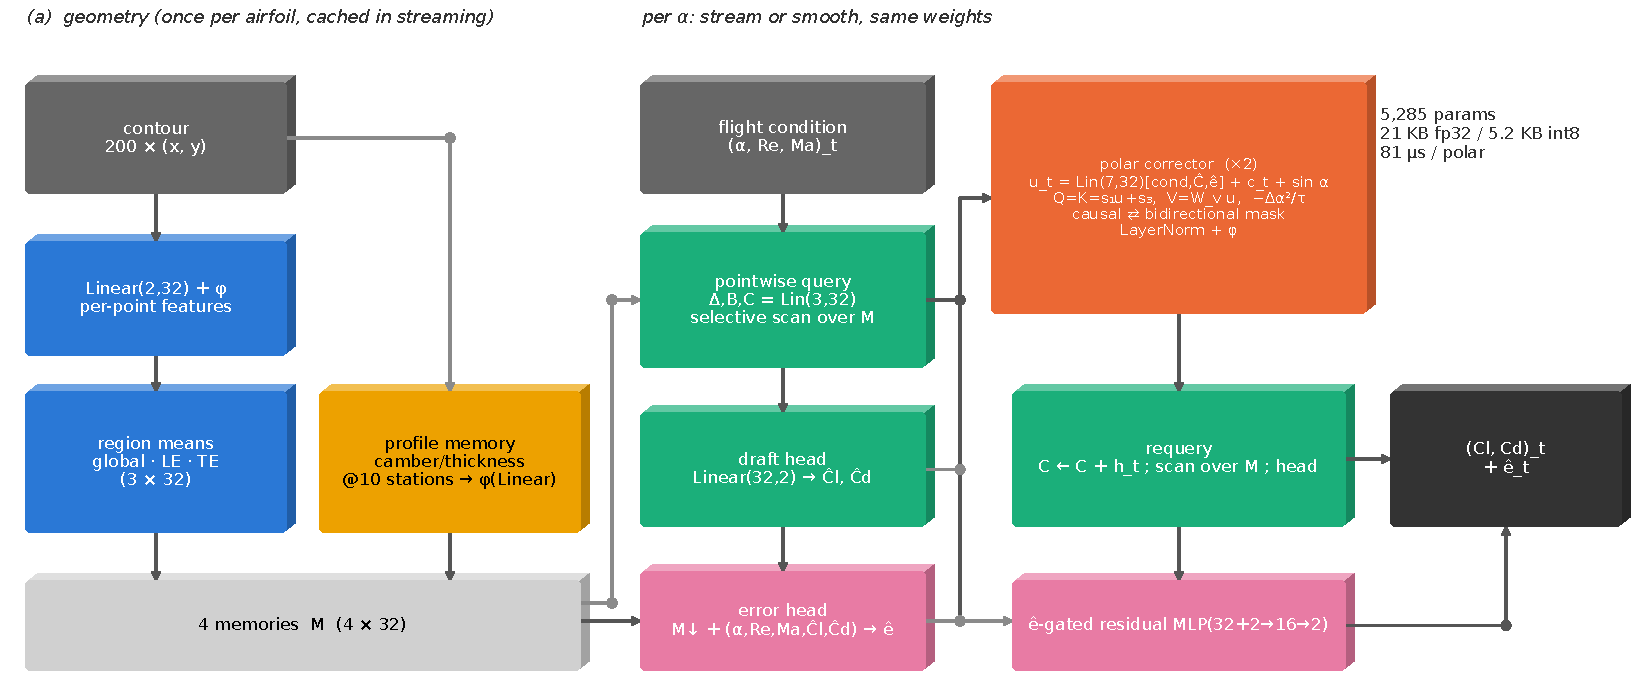
\includegraphics[width=\linewidth]{architecture}
\end{minipage}\hfill
\begin{minipage}[c]{0.28\linewidth}
\centering
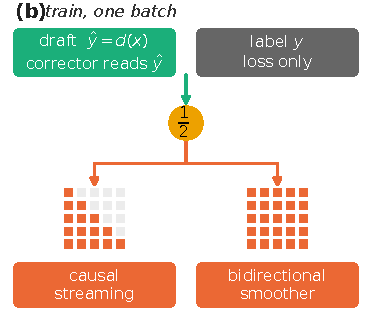
\includegraphics[width=\linewidth]{dualmask}
\end{minipage}
\caption{(a)~FoilCORE. (b)~The corrector reads only $\hat y=d(x)$; each batch is causal or bidirectional with probability $\tfrac12$.}
\label{fig:arch}
\end{figure}

\begin{table}[t]
\centering\footnotesize
\caption{Held-out-geometry test (34,043 polars). Causal AR unless marked. NeuralFoil on a 1,024-polar subset. Latency: $T{=}68$, one CPU thread.}
\label{tab:main}
\setlength{\tabcolsep}{2.0pt}
\begin{tabular}{lrrrrrrl}
\toprule
Model & Params & $C_l$ & $C_d$ (stall) & smooth.\ $C_l$/$C_d$ & MACs/pt & latency & framework \\
\midrule
FoilCORE-5k (ours) & 5,285 & 0.046 & 0.0036 (0.0060) & 0.046 / 0.0036 & 12.8k & 81\,$\mu$s & C++ kernel \\
FoilCORE-2k ($d{=}16$) & 2,373 & 0.057 & 0.0044 (0.0073) & 0.058 / 0.0043 & 6.1k & 61\,$\mu$s & C++ kernel \\
FoilCORE-3k (plain) & 3,434 & 0.076 & 0.0052 (0.0089) & 0.075 / 0.0052 & 11.8k & 67\,$\mu$s & C++ kernel \\
FoilCORE-0.5k ($d{=}8$) & 482 & 0.100 & 0.0083 (0.0129) & 0.100 / 0.0084 & 2.6k & 38\,$\mu$s & C++ kernel \\
3k, label-leaking & 3,434 & 0.137 & 0.0107 (0.0180) & 0.129 / 0.0082 & 11.8k & 68\,$\mu$s & C++ kernel \\
\midrule
\multicolumn{8}{l}{\emph{Same front-end and protocol, standard backbone as corrector:}} \\
\quad Transformer & 5,822 & 0.048 & 0.0037 (0.0061) & 0.047 / 0.0036 & 8.1k & 166\,$\mu$s & C++ kernel \\
\quad TSMixer & 11,780 & 0.061 & 0.0046 (0.0075) & 0.061 / 0.0045 & 2.4k$^{\ast}$ & 50\,$\mu$s & C++ kernel \\
\quad Mamba (S6) & 5,300 & 0.049 & 0.0038 (0.0063) & 0.049 / 0.0038 & 3.7k$^{\ast}$ & 122\,$\mu$s & C++ kernel \\
\midrule
NeuralFoil xxsmall & 13,302 & 0.092 & 0.0128 (0.0256) & -- & 26k & 0.57\,ms & NumPy \\
NeuralFoil xxxlarge & 1,428,166 & 0.082 & 0.0115 (0.0239) & -- & 2.9M & 4.63\,ms & NumPy \\
\bottomrule
\end{tabular}

\end{table}

Task: contour $\{(x_i,y_i)\}_{i=1}^{200}$ and $\{(\alpha_t,\mathrm{Re}_t,\mathrm{Ma}_t)\}_{t=1}^{T}$ ($T\approx 75$) $\rightarrow$ $(C_l,C_d)_t$. Split 80/10/10 by near-duplicate geometry cluster on 5,392 airfoils (XFOIL, ncrit\,=\,9; BigFoil), so test is unseen shapes (539 geometries, 34k polars). Metric: pooled per-point MAE, causal first.

FoilCORE-5k reaches \MainClAR{} $C_l$ / \MainCdAR{} $C_d$ streaming (\SeedN{} seeds \SeedClMean$\pm$\SeedClStd{} / \SeedCdMean$\pm$\SeedCdStd); causal and bidirectional agree to 1\%. NeuralFoil xxxlarge remains 1.2$\times$/1.4$\times$ better in incompressible mid-Re pre-stall; FoilCORE wins overall because it takes Mach and is 2.7--4$\times$ better in stall. With the same front-end and protocol, a transformer (5,822 p) and Mamba (5,300 p) match it; TSMixer (11,780 p) does not. A fused C++ kernel runs a polar in \MainFusedUs\,$\mu$s (0.55\,mJ package-level). Mean-pooled geometry codes collapse to 3--7 principal dimensions; a parameter-free camber/thickness profile as a fourth memory is the largest architectural gain (dropping it: $0.047\rightarrow 0.410$ $C_l$). Analytic lift and drag priors (518 parameters) stack on top of the protocol (next paragraphs). Trained on 10\% of the geometries the same model still reaches 0.081/0.0065. The error head's $C_d$ estimate has Spearman 0.71 with the draft residual and rises 4.8$\times$ on a non-airfoil cloud.

We split by geometry cluster and score the full test set (CSV prefixes are low-Re biased). Per-channel SSM correctors lose to attention; a stall router never fired; depth-3 was worse.

Width $d{=}32$. Each contour point: shared $\mathrm{Linear}(2,d)$ and a per-channel path nonlinearity $\phi$ (Chebyshev series plus a Gaussian bump; pretrained as an autoencoder). Three memories are masked means over the whole contour, leading edge ($x\le 0.25$) and trailing edge ($x\ge 0.75$). The fourth is camber and thickness at ten cosine chord stations (fixed 20-vector, no parameters) mapped by $\mathrm{Linear}(20,d)$ and $\phi$. For every $(\alpha,\mathrm{Re},\mathrm{Ma})$ a selective scan~\citep{gu2024mamba,gu2022s4} over the four memories yields a draft $(\hat C_l,\hat C_d)$; a 16-unit MLP predicts $|\mathrm{draft\ error}|$. Tokens $[\alpha,\mathrm{Re},\mathrm{Ma},\hat C_l,\hat C_d,\hat e]$ plus context and $\mathrm{sinusoid}(\alpha)$ pass two residual-product-attention blocks ($Q{=}K{=}s_1 u+s_3$, $V{=}W_v u$, scores $-\Delta\alpha^2/\tau$, causal or full mask). Loss: MAE on final $+\,0.25\times$ draft MAE ($z$-scored, equal $C_l$/$C_d$) $+\,0.1\times$ error-head L1; AdamW $3\times10^{-4}$, batch 1024, early stopping on causal validation loss. Training: 40\,min per 100 epochs on an RTX A4500.

Three analytic levers add 518 parameters: a potential-flow lift base $2\pi\sin(\alpha-\alpha_0)/\sqrt{1-\mathrm{Ma}^2}$ with a learned stall taper; a fifth memory over six contour scalars plus four boundary-layer scale features; a gated quadratic drag polar. On a second BigFoil pool they are additive over four seeds with complete separation: causal $C_l$ \BaseClAR$\pm$\BaseClStd{} $\rightarrow$ \PhysClAR$\pm$\PhysClStd. Seeded with one measured point, the first causal step beats the physics-free twin's full smoothing pass. They do not transfer zero-shot across pools (normalization uses training-pool statistics); replication retrains per pool.

\section{Limitations}
\label{sec:limits}
Labels are XFOIL at ncrit\,=\,9. The transfer study tests protocol ordering with one small model per dataset, not each dataset's literature; the foundation-model rows are zero-shot on a different information set. Ablation rows are single runs; the main model is three seeds.

Train the refinement stage on the model's own outputs, in both masks, and the deployment mode stops being a compromise.

{\footnotesize\setlength{\bibsep}{2pt}
\bibliographystyle{plainnat}
\bibliography{../references}}

\end{document}
